\documentclass{beamer}
\usetheme{moloch}

\usepackage[czech,english]{babel}
\usepackage{booktabs}
\usepackage{graphicx}
\usepackage{tikz}

\title{NAC-COLORINGS SEARCH\@:\newline COMPLEXITY AND ALGORITHMS}
\author{Petr Laštovička}
\institute{Czech Technical University, Faculty of Information Technology}
\date{June 19, 2025}


%%%%%%%%%%%%%%%
%% Tikz
%%%%%%%%%%%%%%%
\colorlet{ecol}{black!50!white}
\definecolor{colR}{rgb}{.932,.172,.172} %x11 Firebrick2
\definecolor{colB}{rgb}{.255,.41,.884} %svgnames RoyalBlue
\definecolor{colOrange}{RGB}{255,191,0} %Amber
%% Tikz styles
\tikzstyle{vertex}=[circle, draw, fill=black, inner sep=0pt, minimum size=4pt]
\tikzstyle{fvertex}=[circle, draw, fill=white, inner sep=0pt, minimum size=4pt]
\tikzstyle{vertexSig}=[circle, draw, fill=colOrange, inner sep=0pt, minimum size=4pt]
\tikzstyle{edge}=[line width=1.5pt,ecol]
% dotted, densely dotted, loosely dotted, dashed
\tikzstyle{dots}=[dotted dash=1.5pt]
\tikzstyle{redge}=[edge,colR]
\tikzstyle{bedge}=[edge,colB]
\tikzstyle{yedge}=[edge,colOrange]
%%%%%%%%%%%%%%%


\begin{document}
\maketitle

% \section{Goals}
\begin{frame}
	\frametitle{Goals}
	\begin{itemize}
		\item
		      Study basics of Rigidity theory and flexible realizations.
		\item
		      Show that NAC-coloring existence is NP-complete on graphs with maximum degree five.
		\item
		      Design, implement and evaluate an algorithm and heuristics for NAC-coloring search.
	\end{itemize}
\end{frame}

% \section{Rigidity theory}
\begin{frame}
	\frametitle{NAC-coloring}
	\begin{itemize}
		\item
		      \emph{NAC-coloring} is an edge coloring by red and blue such that it is surjective and there are no cycles with exactly one red or blue edge.
		\item
		      It is NP-complete to decide if a graph has a NAC-coloring.
		\item
		      Certifiable by connected components search.
	\end{itemize}
\end{frame}

\begin{frame}
	\frametitle{Flexible realizations}
	\begin{itemize}
		\item
		      Realization of a graph into the space is flexible if it can be transformed while preserving edge lengths, otherwise it is rigid.
		\item
		      Generically rigid graphs may still have some flexible realizations.
		\item
		      A graph has a flexible realization iff.\ there exist a NAC-coloring of the graph.
	\end{itemize}
	\begin{figure}[ht]
		\centering
		\begin{tikzpicture}[rotate=90,scale=1.5]
			\node[vertex] (a) at (0,0) {};
			\node[vertex] (b) at (1,0) {};
			\node[vertex] (c) at (0.5,0.5) {};
			\node[vertex] (d) at (0,1.5) {};
			\node[vertex] (e) at (1,1.5) {};
			\node[vertex] (f) at (0.5,1) {};
			\draw[bedge] (a)edge(b) (b)edge(c) (c)edge(a) (d)edge(e) (e)edge(f) (f)edge(d) ;
			\draw[redge] (a)edge(d) (b)edge(e) (c)edge(f);
		\end{tikzpicture}
		\qquad
		\qquad
		\begin{tikzpicture}[rotate=90,scale=1.5]
			\node[vertex] (a) at (0.00,0) {};
			\node[vertex] (b) at (1.00,0) {};
			\node[vertex] (c) at (0.50,0.5) {};
			\node[vertex] (d) at (0.25,1) {};
			\node[vertex] (e) at (1.25,1) {};
			\node[vertex] (f) at (0.75,1.5) {};
			\draw[edge] (a)edge(b) (b)edge(c) (c)edge(a) (d)edge(e) (e)edge(f) (f)edge(d) ;
			\draw[edge] (a)edge(d) (b)edge(e) (c)edge(f);
		\end{tikzpicture}
	\end{figure}
\end{frame}

\begin{frame}
	\frametitle{NP-comp. \& degree five}
	\begin{itemize}
		\item
		      It has been already known that it is
		\item
		      NP-complete to decide whether a graph has a NAC-coloring.
		\item
		      We show that it is NP-complete to answer also for graphs with maximum degree five. Reduction from 3-SAT.
	\end{itemize}
\end{frame}

\begin{frame}
	\frametitle{Reduction from 3-SAT}

	\begin{figure}[h]
		\centering
		\begin{tikzpicture}[scale=1.50]
			% for~i in~range(1,8):
			%       for~j in~range(1,5):
			%           print(f"\\node[vertex] ({i}{j}) at ({i/2}, {j/2}) {{}};")
			% \node[vertex] (11) at (0.5, 0.5) {};
			\node[vertex]      (22) at (1.25, 1.00) {};
			\node[]           (d22) at (1.00, 1.00) {};
			\node[vertex]      (23) at (1.25, 1.50) {};
			\node[]           (d23) at (1.00, 1.50) {};
			\node[vertex]      (32) at (1.50, 1.00) {};
			\node[vertex]      (33) at (1.50, 1.50) {};
			\node[vertex]      (42) at (2.00, 1.00) {};
			\node[vertex]      (43) at (2.00, 1.50) {};
			\node[vertexSig]   (44) at (2.00, 1.75) {};
			\node[vertex]      (45) at (2.00, 2.25) {};
			\node[vertex]      (46) at (2.00, 2.50) {};
			\node[]           (d46) at (2.00, 2.75) {};
			\node[vertex]      (52) at (2.50, 1.00) {};
			\node[vertex]      (53) at (2.50, 1.50) {};
			\node[vertexSig]   (54) at (2.50, 1.75) {};
			\node[vertex]      (55) at (2.50, 2.25) {};
			\node[vertex]      (56) at (2.50, 2.50) {};
			\node[]           (d56) at (2.50, 2.75) {};
			\node[vertex]      (62) at (3.00, 1.00) {};
			\node[vertex]      (63) at (3.00, 1.50) {};
			\node[vertex]      (72) at (3.25, 1.00) {};
			\node[]           (d72) at (3.50, 1.00) {};
			\node[vertex]      (73) at (3.25, 1.50) {};
			\node[]           (d73) at (3.50, 1.50) {};
			\node[vertex] (special) at (2.25, 0.75) {};

			\node[] at (2.25, 1.5) {$A_i$};

			%%% Left part
			% Bridge to center
			\draw[edge] (32)edge(42) (33)edge(43) (32)edge(33) (32)edge(43);
			\draw[edge] (22)edge(32) (23)edge(33) (22)edge(23) (22)edge(33);
			% Center
			\draw[edge] (32)edge(special) (42)edge(special) (33)edge(44) (43)edge(44) (42)edge(43);
			%%% Decoration
			\draw[edge] (22)edge(d22) (23)edge(d23);
			\node[] at (1.0, 1.25) {$x_i$};
			\node[] at (2.125, 1.25) {$x_i$};

			%%% Right part
			% Bridge to center
			\draw[edge] (52)edge(62) (53)edge(63) (62)edge(63) (53)edge(62);
			\draw[edge] (62)edge(72) (63)edge(73) (72)edge(73) (63)edge(72);
			% Center
			\draw[edge] (62)edge(special) (52)edge(special) (63)edge(54) (53)edge(54) (52)edge(53);
			% Decoration
			\draw[edge] (72)edge(d72) (73)edge(d73);
			\node[] at (3.50,  1.25) {$\bar{x}_i$};
			\node[] at (2.375, 1.25) {$\bar{x}_i$};

			%%% Center piece
			% Center peace and the~one above
			\draw[bedge] (44)edge(45) (54)edge(55) (44)edge(55);
			\draw[bedge] (45)edge(46) (55)edge(56) (45)edge(56);
			\draw[bedge] (44)edge(54) (45)edge(55) (46)edge(56);
			%%% Decoration
			\draw[bedge] (46)edge(d46) (56)edge(d56);
			\node[] at (2.25, 2.75)  {$t$};
			\node[] at (2.25, 1.875) {$t$};

			\begin{scope}[xshift=4cm]
				\node[vertex]    (13) at (0.75, 1.50) {};
				\node[]         (d13) at (0.50, 1.50) {};
				\node[vertex]    (14) at (0.75, 2.00) {};
				\node[]         (d14) at (0.50, 2.00) {};
				\node[vertex]    (23) at (1.00, 1.50) {};
				\node[vertex]    (24) at (1.00, 2.00) {};
				\node[vertex]    (31) at (1.50, 0.75) {};
				\node[]         (d31) at (1.50, 0.50) {};
				\node[vertex]    (32) at (1.50, 1.00) {};
				\node[vertexSig] (33) at (1.50, 1.50) {};
				\node[vertexSig] (34) at (1.50, 2.00) {};
				\node[vertex]    (35) at (1.50, 2.50) {};
				\node[vertex]    (36) at (1.50, 2.75) {};
				\node[]         (d36) at (1.50, 3.00) {};
				\node[vertex]    (41) at (2.00, 0.75) {};
				\node[]         (d41) at (2.00, 0.50) {};
				\node[vertex]    (42) at (2.00, 1.00) {};
				\node[vertexSig] (43) at (2.00, 1.50) {};
				\node[vertexSig] (44) at (2.00, 2.00) {};
				\node[vertex]    (45) at (2.00, 2.50) {};
				\node[vertex]    (46) at (2.00, 2.75) {};
				\node[]         (d46) at (2.00, 3.00) {};
				\node[vertex]    (53) at (2.50, 1.50) {};
				\node[vertex]    (54) at (2.50, 2.00) {};
				\node[vertex]    (63) at (2.75, 1.50) {};
				\node[]         (d63) at (3.00, 1.50) {};
				\node[vertex]    (64) at (2.75, 2.00) {};
				\node[]         (d64) at (3.00, 2.00) {};

				%%% Center
				\draw[edge] (33)edge(34);
				\draw[edge] (43)edge(44);
				\draw[bedge] (34)edge(44);
				\draw[redge] (33)edge(43);
				%%% Labels
				\node[] at (1.750, 1.750) {$B_i$};
				\node[] at (1.375, 1.700) {$x_i$};
				\node[] at (2.125, 1.800) {$\bar{x}_i$};
				\node[] at (1.700, 2.125) {$t$};
				\node[] at (1.800, 1.375) {$f$};

				%%% Left
				\draw[edge] (23)edge(33) (24)edge(34) (23)edge(24) (23)edge(34);
				\draw[edge] (13)edge(23) (14)edge(24) (13)edge(14) (13)edge(24);
				\draw[edge] (13)edge(d13) (14)edge(d14);
				\node[] at (0.50, 1.75) {$x_i$};

				%%% Right
				\draw[edge] (43)edge(53) (44)edge(54) (53)edge(54) (43)edge(54);
				\draw[edge] (53)edge(63) (54)edge(64) (63)edge(64) (53)edge(64);
				\draw[edge] (63)edge(d63) (64)edge(d64);
				\node[] at (3.00, 1.75) {$\bar{x}_i$};

				%%% Top
				\draw[bedge] (34)edge(35) (44)edge(45) (35)edge(45) (35)edge(44);
				\draw[bedge] (35)edge(36) (45)edge(46) (36)edge(46) (36)edge(45);
				\draw[bedge] (36)edge(d36) (46)edge(d46);
				\node[] at (1.75, 3.00) {$t$};

				%%% Bottom
				\draw[redge] (32)edge(33) (42)edge(43) (32)edge(42) (33)edge(42);
				\draw[redge] (31)edge(32) (41)edge(42) (31)edge(41) (32)edge(41);
				\draw[redge] (31)edge(d31) (41)edge(d41);
				\node[] at (1.75, 0.50) {$f$};

			\end{scope}
		\end{tikzpicture}
	\end{figure}

	\vfill

	\begin{figure}[h]
		\centering
		\begin{tikzpicture}[scale=1.50]
			%%% Center
			\node[vertexSig] (35) at (1.5, 2.5) {};
			\node[vertexSig] (53) at (2.5, 1.5) {};
			\node[vertex]    (57) at (2.5, 3.5) {};
			\node[vertex]    (75) at (3.5, 2.5) {};
			\node[] at (2.5, 2.5) {$C_i$};

			%%%%%%%%%%%%%%%%%%%%%%%%%%%%%%%%%%%%%%%%%%%%%%%%%%%%%%%%%%%%%%%%%%%%%%%%%%%%
			%%% t
			%%%%%%%%%%%%%%%%%%%%%%%%%%%%%%%%%%%%%%%%%%%%%%%%%%%%%%%%%%%%%%%%%%%%%%%%%%%%
			\node[vertex] (13) at (0.5, 1.5) {};
			\node[vertex] (14) at (0.5, 2.0) {};
			\node[vertex] (23) at (1.0, 1.5) {};
			\node[vertex] (24) at (1.0, 2.0) {};
			\draw[bedge] (13)edge(23) (14)edge(24) (13)edge(14) (23)edge(24) (13)edge(24);
			\draw[bedge] (53)edge(35) (53)edge(23) (35)edge(24) (53)edge(24);
			%%%% Extensions
			\node[] (13d) at (0.25, 1.5 ) {};
			\node[] (14d) at (0.25, 2.0 ) {};
			\draw[bedge] (13)edge(13d) (14)edge(14d);
			%%%% Labels
			\node[] at (0.25, 1.75) {$t$};
			\node[] at (2.125, 2.125) {$t$};

			%%%%%%%%%%%%%%%%%%%%%%%%%%%%%%%%%%%%%%%%%%%%%%%%%%%%%%%%%%%%%%%%%%%%%%%%%%%%
			%%% x_1
			%%%%%%%%%%%%%%%%%%%%%%%%%%%%%%%%%%%%%%%%%%%%%%%%%%%%%%%%%%%%%%%%%%%%%%%%%%%%
			\node[vertex]    (06)   at (0.25, 3.0 ) {};
			\node[vertex]    (07)   at (0.25, 3.5 ) {};
			\node[vertexSig] (16)   at (0.5 , 3.0 ) {};
			\node[vertexSig] (17)   at (0.5 , 3.5 ) {};
			\node[vertexSig] (26)   at (1.25, 3.0 ) {};
			\node[vertexSig] (27)   at (1.25, 3.5 ) {};
			\node[vertex]    (36)   at (1.5 , 3.0 ) {};
			\node[vertex]    (37)   at (1.5 , 3.5 ) {};
			\node[vertex]    (46)   at (2.0 , 3.0 ) {};
			\node[vertexSig] (p1m1) at (1.0,  3.25) {}; % prism x_1 middle
			\node[vertexSig] (p1m2) at (0.75, 3.25) {};
			\node[vertex]    (p1t1) at (1.0,  2.75) {}; % prism x_1 true
			\node[vertex]    (p1t2) at (0.75, 2.75) {};
			%%%% Construction
			\draw[edge] (35)edge(46) (46)edge(57) (57)edge(37) (36)edge(37) (46)edge(37);
			\draw[edge] (37)edge(27) (36)edge(26) (37)edge(26) (35)edge(36) (46)edge(36) (27)edge(26);
			%%%% Prism
			\draw[bedge] (26)edge(16) (27)edge(17); % linking horizontal edges
			\draw[edge] (26)edge(p1m1) (27)edge(p1m1); % left triangle
			\draw[edge] (16)edge(p1m2) (17)edge(p1m2); % right triangle
			\draw[bedge] (p1m1)edge(p1m2) (p1t1)edge(p1t2);
			\draw[bedge] (p1m1)edge(p1t1) (p1m2)edge(p1t2) (p1m1)edge(p1t2);
			%%%% Train
			\draw[edge] (16)edge(17) (06)edge(07); % vertical
			\draw[edge] (16)edge(06) (17)edge(07); % horizontal
			\draw[edge] (16)edge(07); % diagonal
			%%%% Extensions
			\node[] (06d) at (0.0 , 3.0) {};
			\node[] (07d) at (0.0 , 3.5) {};
			\draw[edge] (07)edge(07d) (06)edge(06d);
			\node[] (p1t1d) at (1.0 , 2.5) {};
			\node[] (p1t2d) at (0.75, 2.5) {};
			\draw[bedge] (p1t1)edge(p1t1d) (p1t2)edge(p1t2d);
			%%%% Labels
			\node[] at (1.875, 2.625) {$\hat{x}_1$};
			\node[] at (2.375, 3.125) {$\hat{x}_1$};
			\node[] at (0.0  , 3.25 ) {$\hat{x}_1$};
			\node[] at (0.875, 2.625) {$t$};


			%%%%%%%%%%%%%%%%%%%%%%%%%%%%%%%%%%%%%%%%%%%%%%%%%%%%%%%%%%%%%%%%%%%%%%%%%%%%
			%%% x_2
			%%%%%%%%%%%%%%%%%%%%%%%%%%%%%%%%%%%%%%%%%%%%%%%%%%%%%%%%%%%%%%%%%%%%%%%%%%%%
			\node[vertex]    (66)   at (3.0 , 3.0 ) {};
			\node[vertex]    (76)   at (3.5 , 3.0 ) {};
			\node[vertex]    (77)   at (3.5 , 3.5 ) {};
			\node[vertexSig] (86)   at (3.75, 3.0 ) {};
			\node[vertexSig] (87)   at (3.75, 3.5 ) {};
			\node[vertexSig] (96)   at (4.5 , 3.0 ) {};
			\node[vertexSig] (97)   at (4.5 , 3.5 ) {};
			\node[vertex]    (A6)   at (4.75, 3.0 ) {};
			\node[vertex]    (A7)   at (4.75, 3.5 ) {};
			\node[vertexSig] (p2m1) at (4.0,  3.25) {}; % prism 2 middle
			\node[vertexSig] (p2m2) at (4.25, 3.25) {};
			\node[vertex]    (p2t1) at (4.0,  2.75) {}; % prism 2 true
			\node[vertex]    (p2t2) at (4.25, 2.75) {};
			%%%% Construction
			\draw[edge] (75)edge(66) (66)edge(57) (57)edge(77) (76)edge(77) (66)edge(77);
			\draw[edge] (77)edge(87) (76)edge(86) (77)edge(86) (75)edge(76) (66)edge(76) (87)edge(86);
			%%%% Prism
			\draw[bedge] (86)edge(96) (87)edge(97); % linking horizontal edges
			\draw[edge] (86)edge(p2m1) (87)edge(p2m1); % left triangle
			\draw[edge] (96)edge(p2m2) (97)edge(p2m2); % right triangle
			\draw[bedge] (p2m1)edge(p2m2) (p2t1)edge(p2t2);
			\draw[bedge] (p2m1)edge(p2t1) (p2m2)edge(p2t2) (p2m1)edge(p2t2);
			%%%% Train
			\draw[edge] (96)edge(97) (A6)edge(A7); % vertical
			\draw[edge] (96)edge(A6) (97)edge(A7); % horizontal
			\draw[edge] (96)edge(A7); % diagonal
			%%%% Extensions
			\node[] (A6d) at (5.0 , 3.0) {};
			\node[] (A7d) at (5.0 , 3.5) {};
			\draw[edge] (A7)edge(A7d) (A6)edge(A6d);
			\node[] (p2t1d) at (4.0 , 2.5) {};
			\node[] (p2t2d) at (4.25, 2.5) {};
			\draw[bedge] (p2t1)edge(p2t1d) (p2t2)edge(p2t2d);
			%%%% Labels
			\node[] at (2.625, 3.125) {$\hat{x}_2$};
			\node[] at (3.125, 2.625) {$\hat{x}_2$};
			\node[] at (5.00 , 3.25 ) {$\hat{x}_2$};
			\node[] at (4.125, 2.625) {$t$};

			%%%%%%%%%%%%%%%%%%%%%%%%%%%%%%%%%%%%%%%%%%%%%%%%%%%%%%%%%%%%%%%%%%%%%%%%%%%%
			%%% x_3
			%%%%%%%%%%%%%%%%%%%%%%%%%%%%%%%%%%%%%%%%%%%%%%%%%%%%%%%%%%%%%%%%%%%%%%%%%%%%
			\node[vertex]    (64)   at (3.0 , 2.0 ) {};
			\node[vertex]    (74)   at (3.5 , 2.0 ) {};
			\node[vertex]    (73)   at (3.5 , 1.5 ) {};
			\node[vertexSig] (84)   at (3.75, 2.0 ) {};
			\node[vertexSig] (83)   at (3.75, 1.5 ) {};
			\node[vertexSig] (94)   at (4.5 , 2.0 ) {};
			\node[vertexSig] (93)   at (4.5 , 1.5 ) {};
			\node[vertex]    (A4)   at (4.75, 2.0 ) {};
			\node[vertex]    (A3)   at (4.75, 1.5 ) {};
			\node[vertexSig] (p3m1) at (4.0,  1.75) {}; % prism 3 middle
			\node[vertexSig] (p3m2) at (4.25, 1.75) {};
			\node[vertex]    (p3t1) at (4.0,  2.25) {}; % prism 3 true
			\node[vertex]    (p3t2) at (4.25, 2.25) {};
			%%%% Construction
			\draw[edge] (75)edge(64) (64)edge(53) (53)edge(73) (74)edge(73) (64)edge(73);
			\draw[edge] (73)edge(83) (74)edge(84) (73)edge(84) (75)edge(74) (64)edge(74) (83)edge(84);
			%%%% Prism
			\draw[bedge] (84)edge(94) (83)edge(93); % linking horizontal edges
			\draw[edge] (84)edge(p3m1) (83)edge(p3m1); % left triangle
			\draw[edge] (94)edge(p3m2) (93)edge(p3m2); % right triangle
			\draw[bedge] (p3m1)edge(p3m2) (p3t1)edge(p3t2);
			\draw[bedge] (p3m1)edge(p3t1) (p3m2)edge(p3t2) (p3m1)edge(p3t2);
			%%%% Train
			\draw[edge] (94)edge(93) (A4)edge(A3); % vertical
			\draw[edge] (94)edge(A4) (93)edge(A3); % horizontal
			\draw[edge] (94)edge(A3); % diagonal
			%%%% Extensions
			\node[] (A4d) at (5.0 , 2.0) {};
			\node[] (A3d) at (5.0 , 1.5) {};
			\draw[edge] (A3)edge(A3d) (A4)edge(A4d);
			\node[] (p3t1d) at (4.0 , 2.5) {};
			\node[] (p3t2d) at (4.25, 2.5) {};
			\draw[bedge] (p3t1)edge(p3t1d) (p3t2)edge(p3t2d);
			%%%% Labels
			\node[] at (3.125, 2.375) {$\hat{x}_3$};
			\node[] at (2.625, 1.875) {$\hat{x}_3$};
			\node[] at (5.00 , 1.75 ) {$\hat{x}_3$};
			\node[] at (4.125, 2.375) {$t$};

		\end{tikzpicture}
	\end{figure}

\end{frame}

\begin{frame}
	\frametitle{FPT algorithm}
	\begin{itemize}
		\item
		      Algorithms polynomial in graph size with a factor \( f(k) \), where~\( k \) is a graph's parameter.
		\item
		      Algorithm for NAC-coloring counting parametrized by treewidth \( k \).
		\item
		      Treewidth represents similarity of a graph with trees.
		\item
		      Decomposition tree where nodes are bags of vertices\newline{}(vertex cuts) of the original graph.
		\item
		      Dynamic programming on the decomposition tree.
	\end{itemize}
\end{frame}

\begin{frame}
	\frametitle{FPT algorithm}
	\begin{itemize}
		\item
		      Information about connectivity in bags needs to be preserved.
		\item
		      Super-exponential complexity in \( k \), linear in the graph size.
		\item
		      Recursive definition of the cache function.
		\item
		      Additional optimizations proposed and variations discussed.
		\item
		      Not implemented, proved only.
	\end{itemize}
\end{frame}

% \begin{frame}
% 	\frametitle{Stable cuts}
% 	\begin{itemize}
% 		\item
% 		      A \emph{stable cut} is a vertex cut that is also an independent set.
% 		\item
% 		      If a stable cut exists, a NAC-coloring also trivially exists.
% 		\item
% 		      Algorithm for stable cut search in flexible graphs implemented.
% 	\end{itemize}
% \end{frame}

\begin{frame}
	\frametitle{NAC-coloring search}
	\begin{itemize}
		\item
		      Naive approach tries all the colorings.
		\item
		      Triangle connected components evolved into monochromatic classes.
		\item
		      Quick check for small cycles using bit masks.
	\end{itemize}

	\begin{figure}[h]
		\centering
		\begin{tikzpicture}[scale=2]
			\node[vertex] (0) at (0, 0) {};
			\node[vertex] (1) at (1, 0.5) {};
			\node[vertex] (2) at (2, 0) {};
			\node[vertex] (3) at (0.5, 0.866) {};
			\node[vertex] (4) at (1.5, 0.866) {};
			\draw[redge] (0)edge(1) (1)edge(2) (0)edge(3) (1)edge(3) (1)edge(4) (2)edge(4) (3)edge(4)  ;
			\draw[edge]  (0)edge(2)  ;
		\end{tikzpicture}
		\qquad
		\begin{tikzpicture}[scale=2]
			\node[vertex] (0) at (0, 0) {};
			\node[vertex] (1) at (1, 0.5) {};
			\node[vertex] (2) at (2, 0) {};
			\node[vertex] (3) at (0.5, 0.866) {};
			\node[vertex] (4) at (1.5, 0.866) {};
			\node[vertex,label={north:$v$}] (5) at (1, 0) {};
			\draw[redge] (0)edge(1) (1)edge(2) (0)edge(3) (1)edge(3) (1)edge(4) (2)edge(4) (3)edge(4)  ;
			\draw[edge]  (0)edge(5) (2)edge(5)  ;
		\end{tikzpicture}
	\end{figure}

\end{frame}

\begin{frame}
	\frametitle{NAC-coloring search}
	\begin{itemize}
		\item
		      Strategy:
		      \begin{itemize}
			      \item
			            Decompose into smaller subgraphs.
			      \item
			            Find all the NAC-colorings of the subgraphs.
			      \item
			            Choose colorings merge order for the subgraphs.
		      \end{itemize}
		\item
		      Multiple heuristics for each stage.
	\end{itemize}
\end{frame}

\begin{frame}
	\frametitle{Benchmarks}
	\begin{itemize}
		\item
		      Flexible vs.\ minimally rigid vs.\ globally rigid.
		\item
		      Any NAC-coloring / all NAC-colorings / the number of NAC-colorings.
	\end{itemize}
\end{frame}

\begin{frame}
	\frametitle{Graphs with many NAC-colorings}
	\begin{itemize}
		\item
		      Improved naive approach is the fastest for find some NAC-coloring.
		\item
		      Fast for finding any NAC-coloring on over 100 vertex graphs.
		\item
		      Listing all NAC-colorings runs fast enough for 30 vertex graphs,
		      naive approach is slow for small graphs.
	\end{itemize}
\end{frame}

\begin{frame}
	\frametitle{Graphs with no/few NAC-colorings}
	\begin{itemize}
		\item
		      Naive search in not feasible.
		\item
		      Monochromatic classes reduce search space significantly.
		      \begin{itemize}
			      \item Hard to randomly find hard graphs.
		      \end{itemize}
		\item
		      Tens of vertices / monochromatic classes run in few seconds.
	\end{itemize}
\end{frame}

\begin{frame}
	\frametitle{NAC-colorings search}
	\begin{itemize}
		\item
		      Extension of our paper from VýLeT.
		\item
		      Code contributed to PyRigi.
		\item
		      I am ready for your questions and discussion.
	\end{itemize}
\end{frame}

\begin{frame}
	\frametitle{Reviewer's question}
	Is it typically the case that the color classes in a NAC-coloring are balanced with respect to the two colors (especially when the graph has only few NAC-colorings)?

	Or does it often happen (in practice) that there exists some NAC-coloring that is largely biased towards one of the two colors?
\end{frame}

\begin{frame}
	\frametitle{Minimally rigid graphs}
	\begin{columns}
		\column{0.5\textwidth}

		\begin{table}[ht]
			\centering
			\begin{tabular}{r|l}
				\toprule
				\,Metric\,    & \,Value\, \\
				\midrule
				Sample size   & 1000      \\
				NAC-colorings & 1602k     \\
				Weighted avg. & 0.60      \\
				Average       & 0.63      \\
				Std           & 0.21      \\
				Min           & 0.06      \\
				25            & 0.46      \\
				50            & 0.65      \\
				75            & 0.83      \\
				Max           & 0.94      \\
				\bottomrule
			\end{tabular}
		\end{table}

		\column{0.5\textwidth}

		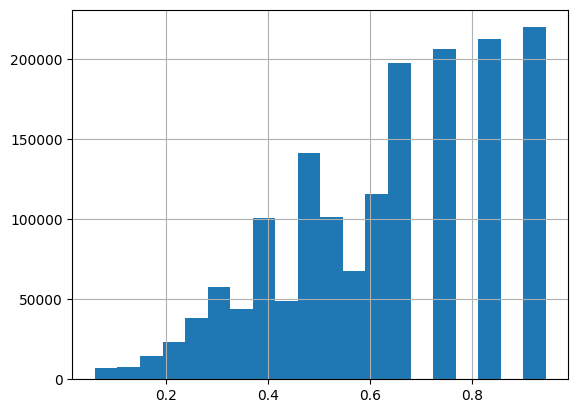
\includegraphics[width=0.9\textwidth]{./assets/presentation_reviewer_minimally_rigid.png}
	\end{columns}

	\centering
	Minimally rigid graphs with 18 to 20 vertices.
\end{frame}

\begin{frame}
	\frametitle{Globally rigid graphs (single)}
	\begin{columns}
		\column{0.5\textwidth}

		\begin{table}[ht]
			\centering
			\begin{tabular}{r|l}
				\toprule
				\,Metric\,    & \,Value\, \\
				\midrule
				Sample size   & 1000      \\
				NAC-colorings & 1000      \\
				Weighted avg. & 0.09      \\
				Average       & 0.09      \\
				Std           & 0.09      \\
				Min           & 0.05      \\
				25            & 0.06      \\
				50            & 0.07      \\
				75            & 0.09      \\
				Max           & 0.85      \\
				\bottomrule
			\end{tabular}
		\end{table}

		\column{0.5\textwidth}

		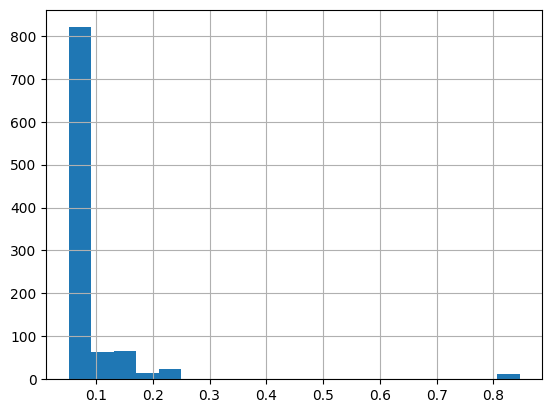
\includegraphics[width=0.9\textwidth]{./assets/presentation_reviewer_globally_rigid_single.png}

	\end{columns}

	\centering
	Globally rigid graphs with 18+ vertices and one unique NAC-coloring.
\end{frame}

\begin{frame}
	\frametitle{Globally rigid graphs (few)}

	\begin{columns}
		\column{0.5\textwidth}

		\begin{table}[ht]
			\centering
			\begin{tabular}{r|l}
				\toprule
				\,Metric\,    & \,Value\, \\
				\midrule
				Sample size   & 1000      \\
				NAC-colorings & 3287      \\
				Weighted avg. & 0.11      \\
				Average       & 0.13      \\
				Std           & 0.11      \\
				Min           & 0.05      \\
				25            & 0.07      \\
				50            & 0.10      \\
				75            & 0.16      \\
				Max           & 1.00      \\
				\bottomrule
			\end{tabular}
		\end{table}

		\column{0.5\textwidth}

		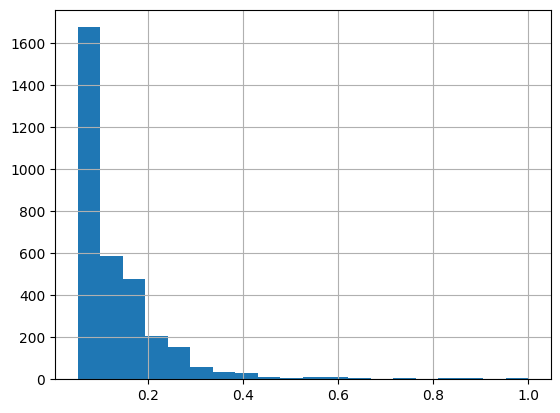
\includegraphics[width=0.9\textwidth]{./assets/presentation_reviewer_globally_rigid_few.png}

	\end{columns}

	\centering
	Globally rigid graphs with 18+ vertices and at most 10 unique NAC-colorings.
\end{frame}

\end{document}
